% Journal Quantum Science and Technology
% Special issue: Focus on Perspectives on the Future of Variational Quantum Computing
% https://iopscience.iop.org/collections/qst-241120-732


\documentclass[12pt]{iopart}

\newcommand{\gguide}{{\it Preparing graphics for IOP Publishing journals}}
%Uncomment next line if AMS fonts required
%\usepackage{iopams}  

\usepackage[hidelinks]{hyperref}
\usepackage{url}
\usepackage{comment}
\usepackage{graphicx}
\usepackage{float}
\usepackage{subfigure}
\usepackage{tabularx}
\usepackage{orcidlink}
\usepackage{cite}
\bibliographystyle{iopart-num}
\usepackage{amsmath}
\usepackage{appendix}



\begin{document}

%\title[Quantum Computing Plasma Dispersion Relations]{Quantum Computing Plasma Dispersion Relations}

\title[Extracting Plasma Dispersion Relations using a Quantum Algorithm]{Extracting Plasma Dispersion Relations using a Quantum Algorithm}


\author{
    Óscar Amaro \orcidlink{0000-0003-0615-0686} $^1$,
    Lucas Gamiz \orcidlink{0000-0002-7393-0896} $^1$, %Lucas Ivan Inigo Gamiz <lucas.inigo.gamiz@tecnico.ulisboa.pt>,
    Efstratios Koukoutsis \orcidlink{0000-0002-9143-2743} $^2$,
    %João Pinto Barros??? \orcidlink{0000-0002-4336-0204} $^3$,
    Marija Vranic \orcidlink{0000-0003-3764-0645} $^1$ %marija.vranic@tecnico.ulisboa.pt
  }

\address{$^1$ GoLP/Instituto de Plasma e Fus\~ao Nuclear, Instituto Superior T\'ecnico, Universidade de Lisboa, Lisbon, Portugal\\
$^2$ School of Electrical and Computer Engineering,
National Technical University of Athens, Zographou 15780, Greece\\
%$^3$ ETHZ, Switzerland
}

%\address{
%GoLP/Instituto de Plasmas e Fus\~{a}o Nuclear, Instituto Superior T\'{e}cnico, Universidade de Lisboa, 1049-001 Lisbon, Portugal
%}
\ead{\footnotesize
\href{mailto:oscar.amaro@tecnico.ulisboa.pt}{oscar.amaro@tecnico.ulisboa.pt}, \href{mailto:marija.vranic@tecnico.ulisboa.pt}{marija.vranic@tecnico.ulisboa.pt}
}\normalsize

\vspace{10pt}

\begin{abstract}
    %Knowledge about wave propagation and instabilities in plasmas is crucial for many applications, including accelerators, nuclear fusion reactors, etc.
    
Understanding wave propagation and instabilities in plasmas is central to both fundamental plasma physics and applications such as nuclear fusion. A key quantity is the dispersion relation, describing how perturbations of frequency and wavenumber $\omega(k)$ propagate or grow. Conventional extraction of dispersion branches relies on root-finding, which can become numerically unstable or costly, especially when many modes are present.

Quantum algorithms have the potential to solve certain classes of eigenvalue problems more efficiently. While methods such as Quantum Phase Estimation and the Rodeo Algorithm \cite{choiRodeoAlgorithmQuantum2021} efficiently recover real spectra of Hermitian Hamiltonians, instabilities require access to complex eigenvalues. To this end, we explore a variational framework \cite{xieVariationalQuantumAlgorithms2024} that encodes non-Hermitian plasma Hamiltonians into measurable Hermitian cost functions, whose minima yield the desired eigenvalues.

As a proof of concept, we apply both classes of algorithms to simple plasma dispersion problems. In the cold two-stream instability, the dynamics can be encoded into a $4\times4$ matrix representing density and velocity perturbations of the beams, from which the quantum algorithm recovers the wave frequency and growth rate. This setup is implementable on present-day quantum hardware. We also investigate more complex scenarios, including multibranch relations, kinetic instabilities \cite{engelQuantumAlgorithmVlasov2019}, and optimizations for Hamiltonian encoding, state preparation, and error mitigation.

These results highlight the potential of quantum approaches for studying plasma dispersion relations, suggesting a pathway toward efficient analysis of high-dimensional kinetic instabilities relevant to fusion research.

\end{abstract}


\section{Introduction}

\textbf{Story bullet-points:}
\begin{itemize}
    \item Plasma Physics and Dispersion Relations
    \item SOTA of classical DR solvers and possible limitations
    \item Formulation of DR as eigenvalue problem 
    \item Quantum Algorithms for eigenvalue problems (Hermitian and non-Hermitian
    \item NISQ-adapted algorithms
\end{itemize}

% NISQ
NISQ implies noise, which require shallow circuits to perform meaningful computations, which usually in practice leads to the use of hybrid-methods.
Variational Quantum Eigensolvers are useful \cite{tillyVariationalQuantumEigensolver2022,fedorovVQEMethodShort2022}


% QPE
Quantum Phase Estimation has been used to compute eigenvalues.
\cite{shaoComputingEigenvaluesDiagonalizable2022}
% Rodeo
However, QPE is usually too expensive to run on NISQ devices for larger systems. Instead, an alternative has been proposed - Rodeo Algorithm.
%
``The Quantum Rodeo Algorithm is a stochastic quantum computing method designed for efficient eigenstate preparation and eigenvalue estimation of quantum Hamiltonians. It stands out for its exponential speed advantage over traditional algorithms like phase estimation and adiabatic evolution, particularly in preparing eigenstates.''
%
The Rodeo algorithm was first introduced in \cite{choiRodeoAlgorithmQuantum2021}. An optimized version in \cite{cohenOptimizingRodeoProjection2023}.
%
It was experimentally demonstrated in \cite{qianDemonstrationRodeoAlgorithm2024}. 
%
It has also been made variational in \cite{zhuEfficientQuantumEstimation2025}, where it is applied to GS and Excited states of a molecule.
%
Other studies include \cite{rochaEstimatingNumberStates2024,gomesUnravelingRodeoAlgorithm2025}.
% Don't know how to include this reference yet, so I wouln't
%The nonlinear dynamics of the TSI can be approximately simulated within a quantum computing formalism \cite{maySecondQuantizationNonlinear2025}
In \cite{engelQuantumAlgorithmVlasov2019}, the authors simulate the real-time evolution of a Hermitian system. This is the linearized ElectroStatic Vlasov 0D1V system.



% non-hermitian
More generally, Plasma Physics Hamiltonians are Non-Hermitian.
% review
Non-Hermitian Physics has Review
\cite{ashidaNonHermitianPhysics2020}
% real-time 
There are some works on quantum simulation of time evolution of non-Hermitian Hamiltonians has been done in \cite{jebraeilliQuantumSimulationQubit2025,zhangObservationExceptionalPoint2021,dograQuantumSimulationParity2021}.
%
Generalized eigenvalue problems have been discussed in \cite{parkerQuantumPhaseEstimation2020,rajchel-mieldziocQuantumAlgorithmSolving2025}
%
Find complex eigenvalues of non-Hermitian Hamiltonians \cite{wangMeasurementbasedQuantumPhase2010,daskinUniversalQuantumCircuit2014,xieVariationalQuantumAlgorithms2024,armaosQuantumComputingAtmospheric2024,liNonHermitianCouplingStrength2025}.
%
In \cite{buczkowskiGlobalRootsPoles2024} the authors use a triangulation method for the search of roots and poles in the complex plane, which could be useful for the study of non-Hermitian Hamiltonians.
%
In \cite{zhaoUniversalVariationalQuantum2023} the authors present experimental results for the eigenanalysis of non‑Hermintian matrices, with explicit ansatze and cost functions, and applied to the stability of a small electric circuit. In \cite{zhangQuantumComputingExtracting2025, singhQuantumSimulationsNuclear2025} the authors apply similar approaches to extract nuclear resonances.
%
In \cite{zhangObservationExceptionalPoint2021} the authors observe exceptional points in a non-Hermitian Hamiltonian, running on a 2-qubit quantum circuit.
%
In \cite{zhangObservingExponentialGrowth2025} the authors don't use quantum circuits but study the eigenmodes of a non-Hermitian RLC resonator electrical circuit spontaneous PT-symmetry breaking.
%
In \cite{yangEndtoEndQuantumEstimation2026} the authors develop a new algorithm built on QSVT to obtain the pseudospectra of non-Hermitian Hamiltonian, using a IonQ QPU.


\section{Methods}

\begin{figure}[!h]
    \centering
    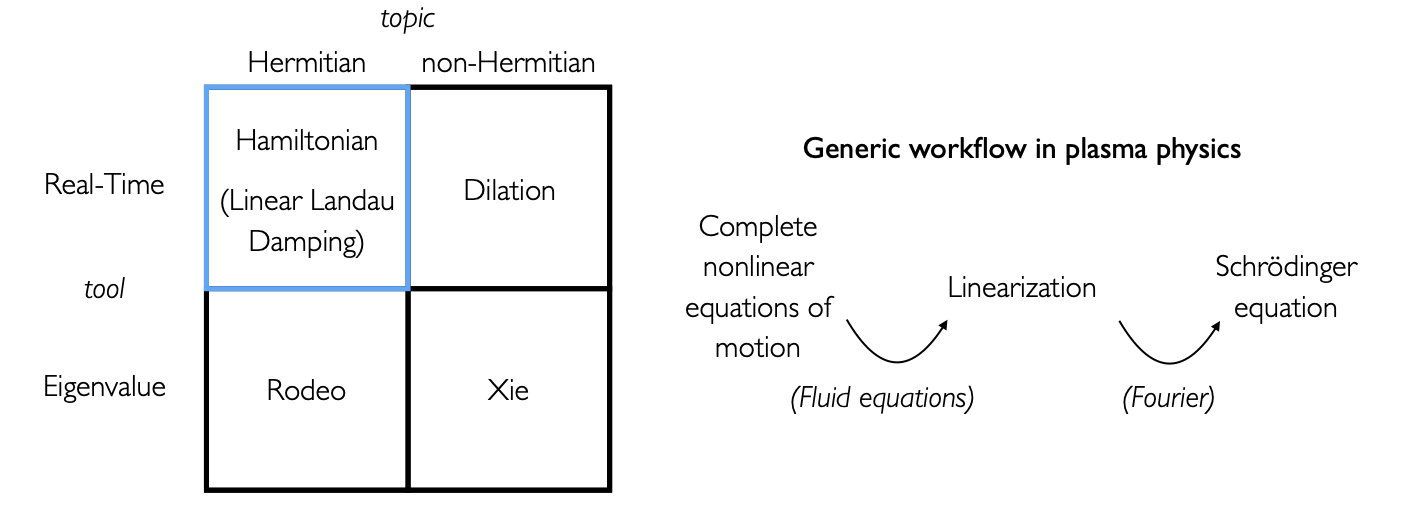
\includegraphics[width=0.7\linewidth]{figures/hamiltonian_classes.png}
    \caption{Caption}
    \label{fig:hamiltonian_classes}
\end{figure}

\subsection{Hermitian Hamiltonians}

\subsection{CMA diagram}

\begin{figure}[!h]
    \centering
    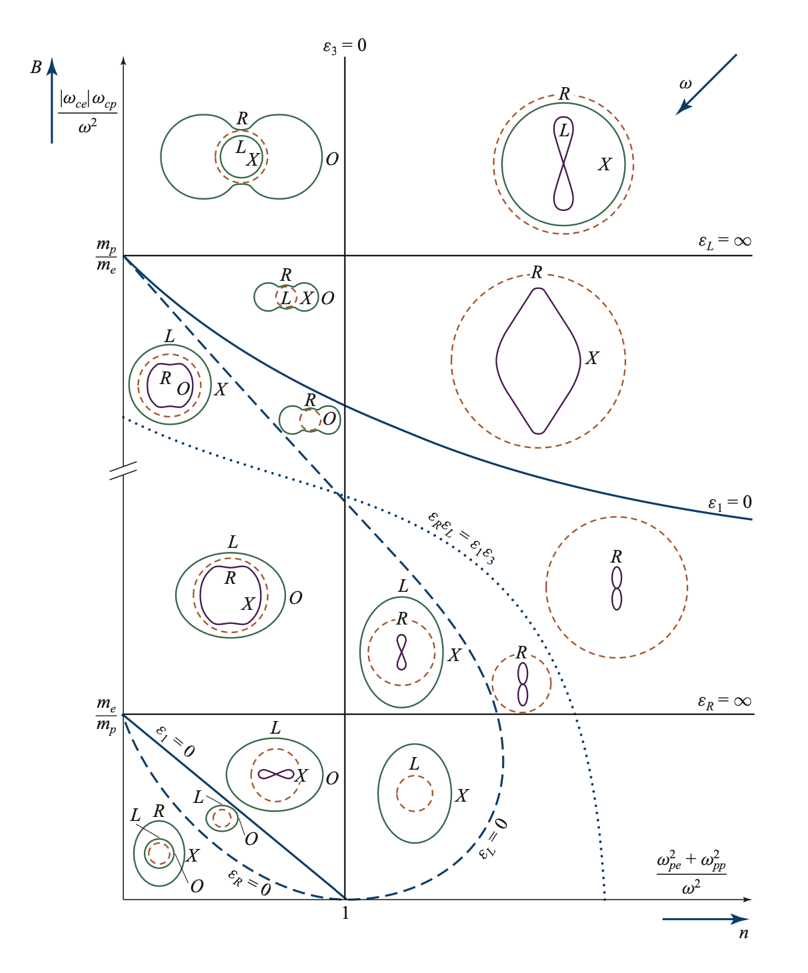
\includegraphics[width=0.5\linewidth]{figures/cma.png}
    \caption{CMA diagram of waves}
    \label{fig:cma}
\end{figure}

\subsection{Non-Hermitian Hamiltonians}

% Hamiltonian structure of the TSI
The Hamiltonian structure of the linear two-stream equation system for a single k was first studied by Kueny and Morrison \cite{kuenyNonlinearInstabilityChaos1995}.

\begin{figure}[!h]
    \centering
    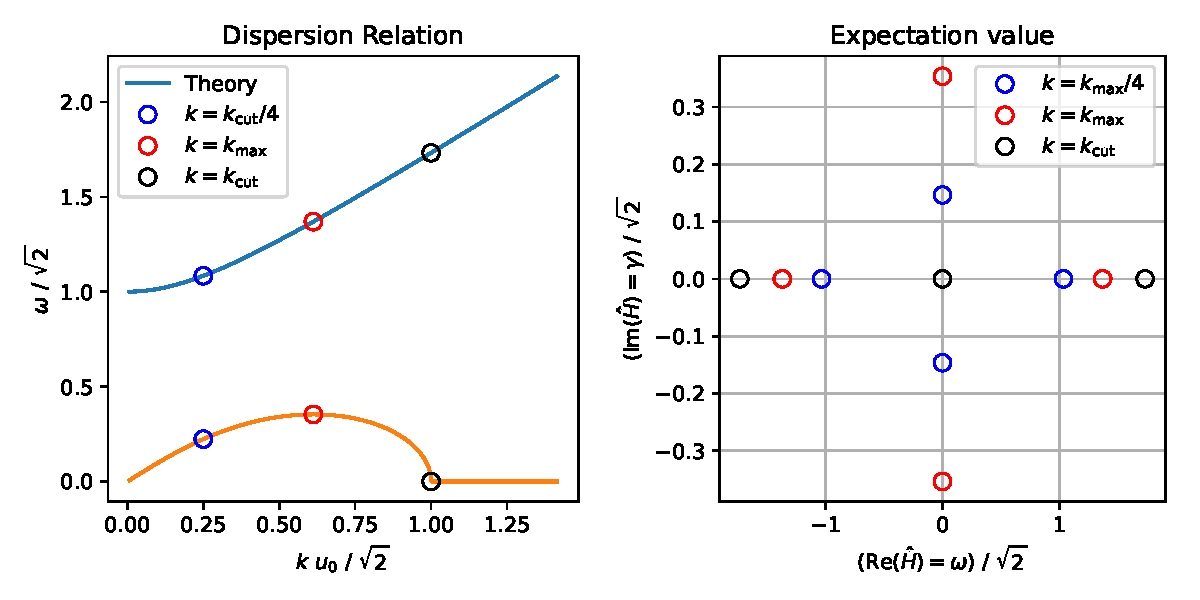
\includegraphics[width=0.7\linewidth]{figures/instabilities_TSI.pdf}
    \caption{Two-Stream Instability}
    \label{fig:instabilities_TSI}
\end{figure}

The “phase-transition” to purely real eigenvalues (stable) hints at some change in entanglement. Indeed, if we track the von-Neumann entanglement entropy $S_{vN}(\rho_A)=-\mathrm{Tr}(\rho_A \log \rho_A)$, where $\rho_A=\mathrm{Tr}_B(|\psi\rangle \langle \psi|)$ along the wavenumber (here sorted), we can see an abrupt change at $k=k_{cut}=\sqrt{2}$. Don’t know why the fluctuations appear at $k \sim \sqrt{2}/2$.
For very low $k$ (high $\lambda$), only one mode is highly entangled/correlated.
For very high $k$ (low $\lambda$), all modes are mostly uncorrelated (no reinforced feedback-loop).

The von-Neumann entanglement entropy cannot be measured directly on a quantum computer.
However, the Rényi entropy of order 2 can be measured through a SWAP protocol (for many qubits this can be long interaction). The proof is relatively simple. See figure \ref{fig:tsi_Renyi}.

\begin{figure}[!h]
    \centering
    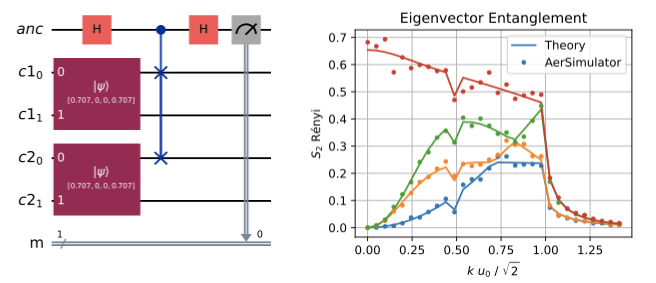
\includegraphics[width=0.7\linewidth]{figures/tsi_Renyi.png}
    \caption{Circuit to measure the Renyi-2 entanglement entropy, and simulated results, showcasing the ``phase-transition''.}
    \label{fig:tsi_Renyi}
\end{figure}






\section{State Preparation}

- the ansatz has to have some structure, sweetspot between classical and quantum
- I suggest that we use ideas from quantum chemistry, like Hartree-Fock initial state preparation as a good initial guess and then use a simpler variational block
- I also suggest building some ground state of the plasma system
- Stratos builds on this and suggests to use unmagnetized solutions to build magnetized. So the strategy could be (T=0,B=0) -> (T=0,B) -> (T,B)



\section{Observable Decomposition}

- Pauli Expansion: divide-and-conquer idea. I actually don't know if the approach is inefficient for general sparse matrices, but I know that the Engel2019 Hamiltonian is dense, so I didn't pursue this


\subsection{Measuring}
- can we build a loss function that is not an observable?

building L coss function from the von-Neumann entropy rho log(rho), which is not an observable and it is very nonlinear on the (mixed) state. Stratos suggests to build an ensemble of polynomials on the states and then get the entropy, but we both agree that this could be complicated



\begin{figure}[!h]
    \centering
    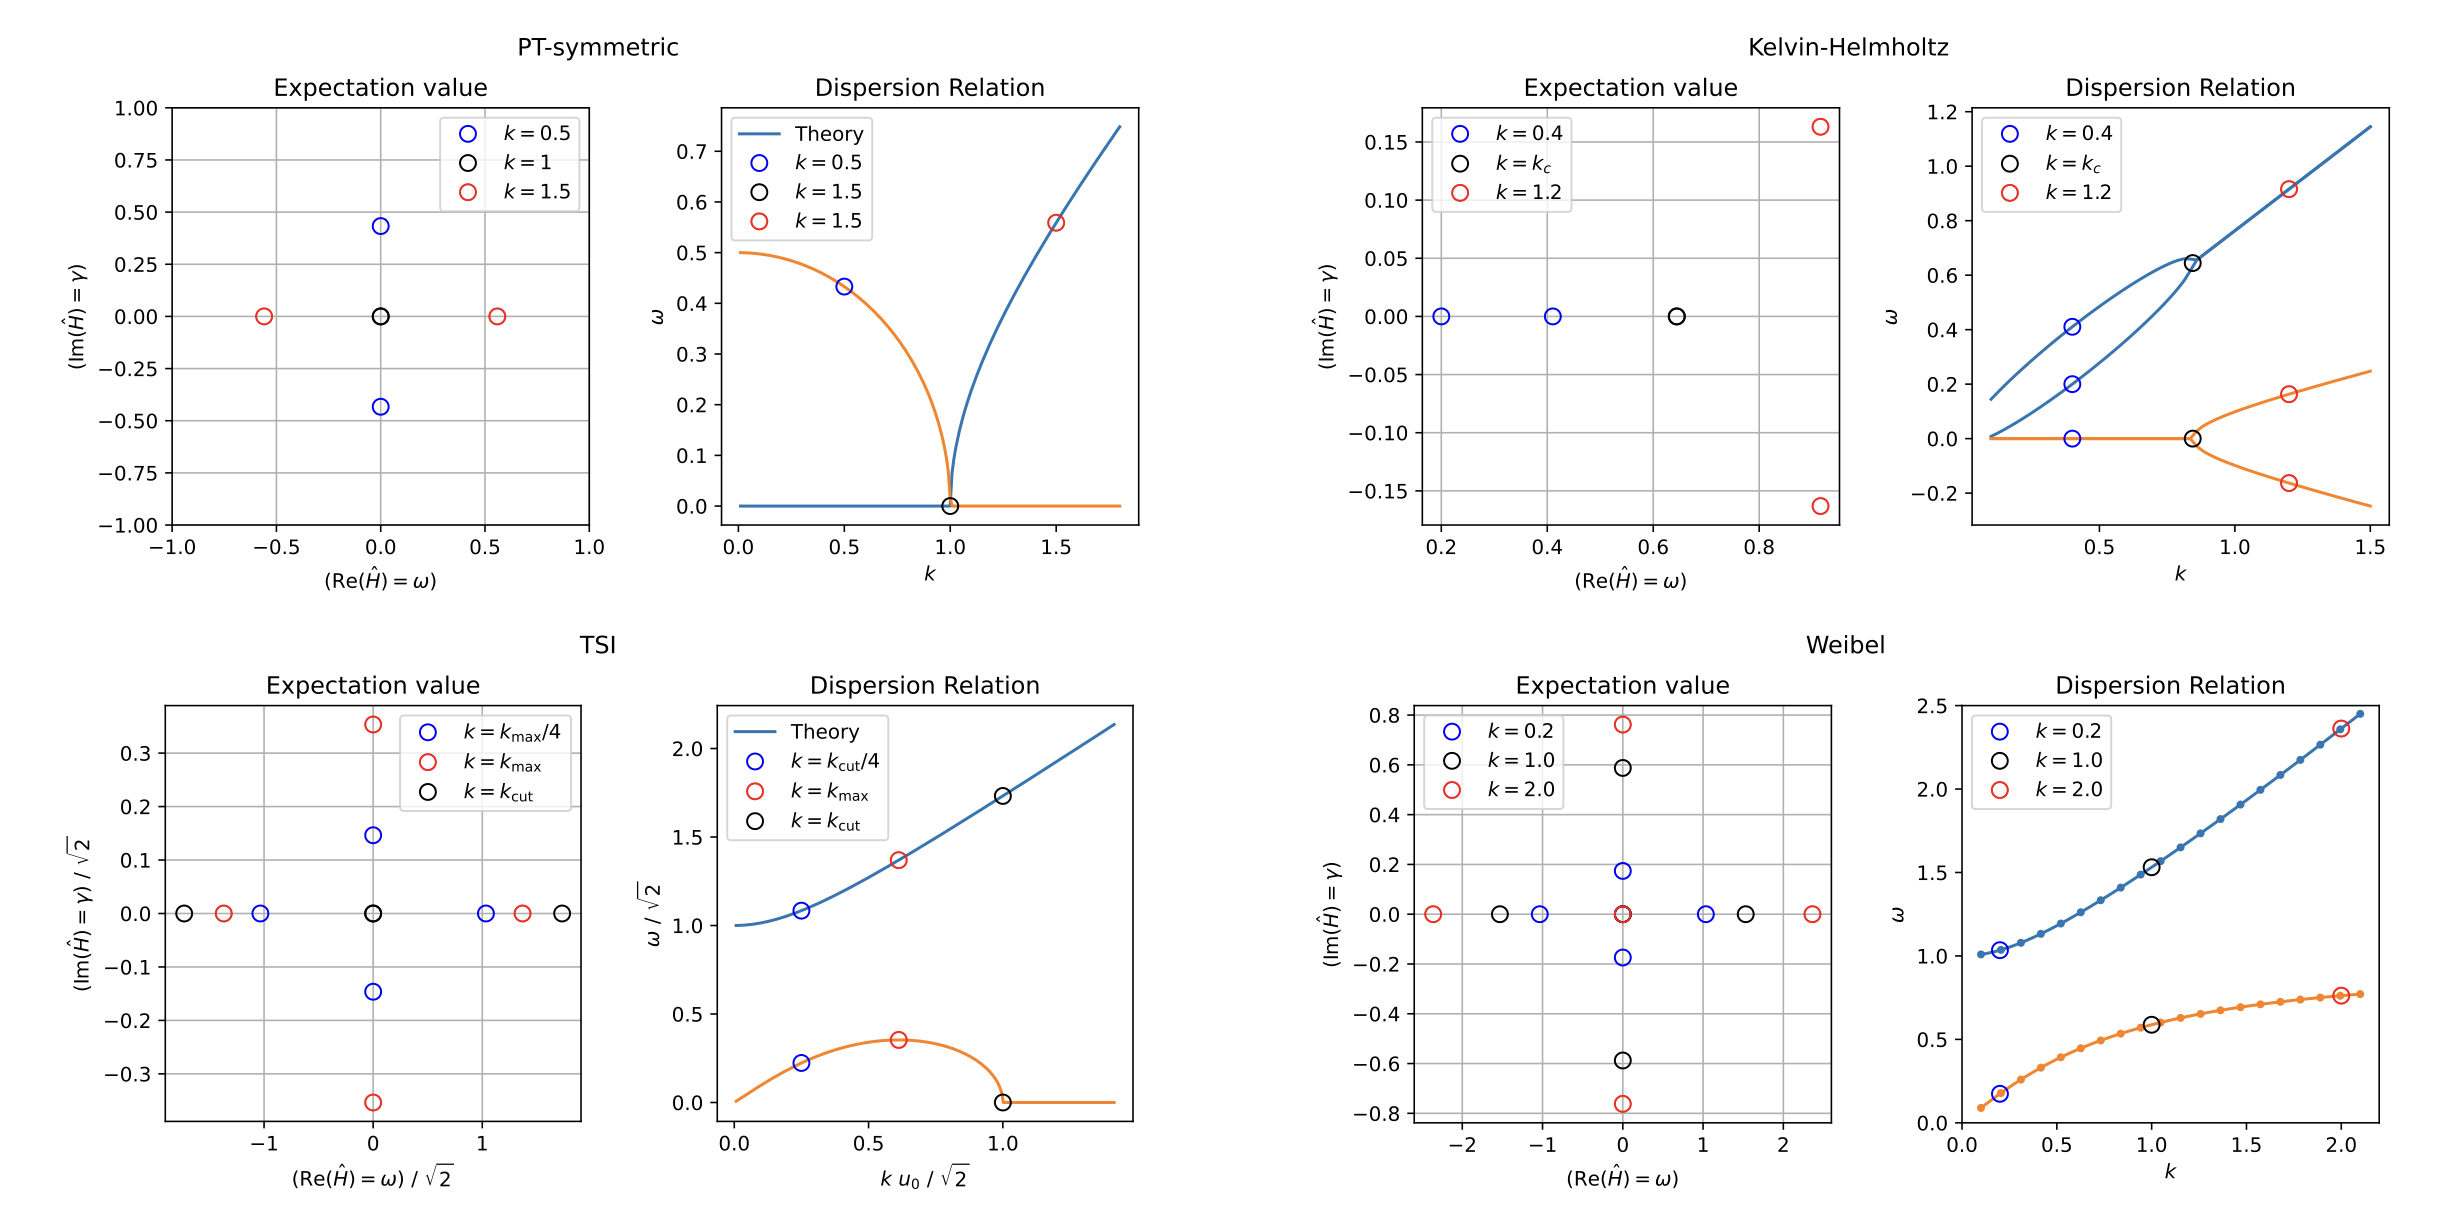
\includegraphics[width=0.8\linewidth]{figures/minimal_examples.png}
    \caption{4 examples}
\end{figure}


\section{Conclusions}

Would the 2D/3D, multispecies, kinetic versions of the Hamiltonians be so high-dimensional that a quantum algorithm with its encoding of the Hamiltonian through Pauli-string or other would be more practical to extract information about the dispersion relation?



\section{Data and Code availability statement}\label{sc:codeavailability}

The data that support the findings of this study are available at \url{https://replasma.github.io/}.

\section{Acknowledgments}\label{sc:acknowledgments}

% 
The authors thank João Pinto Barros for useful discussions on the quantum Rodeo Algorithm, Alexandra Alves on Quantum Phase and Amplitude Estimation, and Filipe Cruz and Ankur Nath on plasma Dispersion Relations.

% The authors thank ..., for fruitful discussions and proofreading the manuscript.

% funding
This work was supported by the European Research Council (ERC-2015-AdG Grant No. 695088) and Portuguese Science Foundation (FCT) Grants No. CEECIND/01906/2018, PTDC/FIS-PLA/3800/2021, and UI/BD/153735/2022.

% computational resources
%We acknowledge the use of IBM Quantum services for this work. In this paper we used ibmq\_vigo, which is one of the IBM Quantum Canary processors. The views expressed are those of the authors, and do not reflect the official policy or position of IBM or the IBM Quantum team.

%We acknowledge PRACE for awarding access to MareNostrum based in the Barcelona Supercomputing Centre. 
We acknowledge the EuroHPC Joint Undertaking for awarding this project access to the EuroHPC supercomputer LUMI, hosted by CSC (Finland) and the LUMI consortium through a EuroHPC Regular Access call. 


Classical simulations were performed at Deucalion HPC Portugal.
%
Quantum simulations ...




\vspace{10pt}
\noindent \textbf{References}
\bibliography{bibtex}


\setcounter{equation}{0}
\renewcommand{\theequation}{A.\arabic{equation}}

\section*{Appendix: PT-symmetric solved example}\label{app:A}

Here we present an example of the variational procedure for the minimal 2x2 PT-symmetric non-Hermitian matrix, which has a fully analytical solution.

The non-Hermitian matrix has eigenvalues and eigenvectors:

\begin{equation}
    \boxed{ H= \dfrac{1}{2}~ \left( \begin{matrix} i \Gamma & k \\ k & -i \Gamma \end{matrix} \right), \quad \lambda_\pm = \pm \dfrac{1}{2} \sqrt{k^2-\Gamma^2}, \quad v_\pm = \left( i\Gamma/k \pm \sqrt{1-\Gamma^2/k^2} ,1 \right) }
\end{equation}

Defining the quadratic Hermitian $M \equiv (H-\epsilon)^\dagger (H-\epsilon)$ with variational energy $\epsilon \equiv \epsilon_r + i \epsilon_i $

\begin{equation}
\boxed{ M = \dfrac{1}{4}~ \left( \begin{matrix}
(\Gamma-2 \epsilon_i)^2 + 4 \epsilon_r^2 + k^2 &
-2i \Gamma k - 4 \epsilon_r k \\
+2i \Gamma k - 4 \epsilon_r k &
(\Gamma + 2 \epsilon_i)^2 + 4 \epsilon_r^2 + k^2 
 \end{matrix} \right) }
\end{equation}

The minimal ansatz for this 1-qubit example is $|\psi(\theta)\rangle = U(\theta)|0\rangle = R_z(\theta_1) ~R_y(\theta_0)~|0\rangle$. This will be enough to approximate the right-eigenvectors of $H$.

Normalizing $\Gamma=1$, we have the closed-form cost function $L=\langle \psi | M| \psi \rangle$

\begin{equation}
    \boxed{ L(\epsilon_r,\epsilon_i,\theta,\phi)= ( 1 + 4 \epsilon_i^2 + 4 \epsilon_r^2 + k^2 - 4 \epsilon_i \cos(\theta) + 2 k \sin(\theta) (\sin(\phi) -2 \epsilon_r \cos(\phi) ) )/4 }
\end{equation}

We can decompose the general form of $M$ into Hermitian and anti-Hermitian operators:

$M(\epsilon) \equiv (H^\dagger - \epsilon^*)(H-\epsilon)=H^\dagger H-\epsilon^*H-\epsilon H^\dagger + |\epsilon|^2= H^\dagger H -(\epsilon_r-i \epsilon_i)H - (\epsilon_r+i\epsilon_i)H^\dagger + \epsilon_r^2+\epsilon_i^2 =  H^\dagger H +\epsilon_r(-H-H^\dagger)+ i \epsilon_i (H-H^\dagger) + \epsilon_r^2+\epsilon_i^2$

We can also compute in closed-form the operators for the gradients of $M$ with respect to the variational energies

\begin{align}
    P_r \equiv \partial_{\epsilon_r} M = -(H+H^\dagger) + 2\epsilon_r I = \left( \begin{matrix} 2 \epsilon_r & -k \\ -k & 2 \epsilon_r \end{matrix} \right) \\
    P_i \equiv \partial_{\epsilon_i} M = i(H-H^\dagger) + 2\epsilon_i I =  \left( \begin{matrix} 2 \epsilon_i-1 & 0 \\ 0 & 2 \epsilon_i-1 \end{matrix} \right)
\end{align}

The Parameter-Shift Rules (PSR) lead to $\partial_\theta L = ( L(\theta+\pi/2) - L(\theta-\pi/2) )/2$ and $\partial_\phi L = ( L(\phi+\pi/2) - L(\phi-\pi/2) )/2$. However, in this simple case we can compute all the gradients explicitly:

\begin{align}
    \partial_{\theta} L = \epsilon_i \sin(\theta) + k \cos(\theta)( \sin(\phi) - 2 \epsilon_r \cos(\phi) )/2
    \\
    \partial_{\phi} L = k \sin(\theta) (\cos(\phi) + 2 \epsilon_r \sin(\phi))/2
    \\
    \partial_{\epsilon_r} L = 2 \epsilon_r - k \cos(\phi) \sin(\theta)
    \\
    \partial_{\epsilon_i} L = 2 \epsilon_i - \cos(\theta)
\end{align}

We can obtain the optimal angles $\theta_\mathrm{opt}=\pi/2$ and solving $\partial_{\phi} L = 0 $ leads to $ \phi_\mathrm{opt} = 3\pi/2+\arctan(2\epsilon_r)$. Replacing these values in the results before

\begin{align}
    L_\mathrm{opt} = \left( 1+4\epsilon_i^2 + 4\epsilon_r^2 - 2k \sqrt{1+4\epsilon_r^2} +k^2 \right) / 4
    \\
    \partial_{\theta} L_\mathrm{opt} = \epsilon_i
    \\
    \partial_{\phi} L_\mathrm{opt} = 0
    \\
    \partial_{\epsilon_r} L_\mathrm{opt} = 2\epsilon_r \left( 1 - k  / \sqrt{1+4\epsilon_r^2} \right)
    \\
    \partial_{\epsilon_r} L_\mathrm{opt} = 2\epsilon_i
\end{align}

We can also decompose the $M$ matrix explicitly into Pauli Strings

\begin{equation}
    M = \dfrac{1 + 4\epsilon_i^2 + 4\epsilon_r^2 + k^2}{4} I - k \epsilon_r ~X + \dfrac{k}{2} ~Y - \epsilon_i ~Z
\end{equation}

for which the $N_{GCP}$ minimal group of commuting Paulis is $3$.


% runs on IBM
We have deployed these observables (cost function and some of its gradients) on IBM QPUs. In figure \ref{fig:ptsym_estimator} we prescribe all the variational parameters (there is no optimization loop).

\begin{figure}[!h]
    \centering
    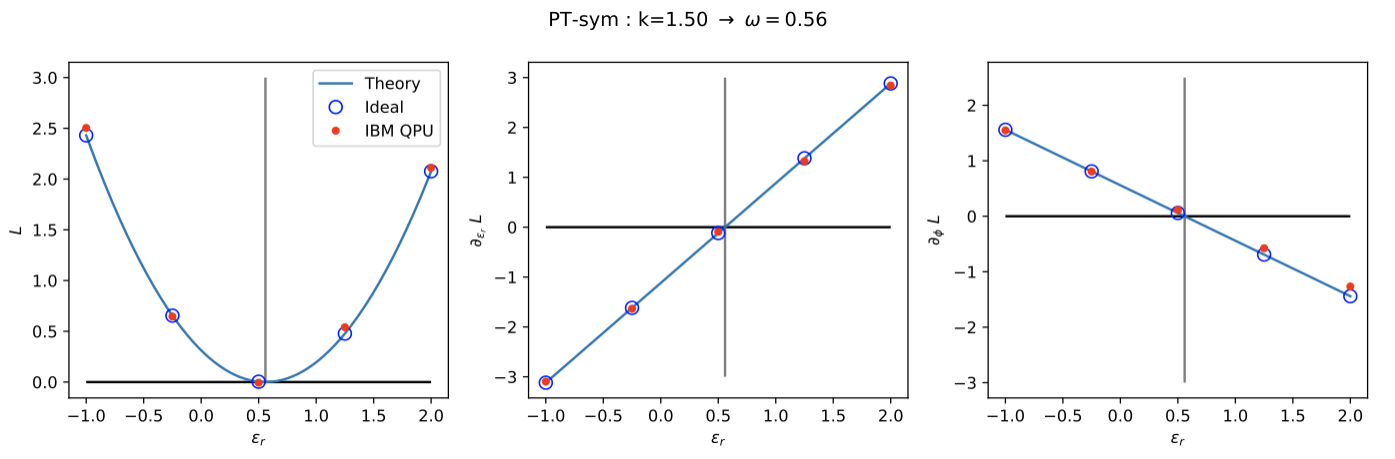
\includegraphics[width=0.8\linewidth]{figures/ptsym_estimator.png}
    \caption{Measurement of observables on IBM QPU.}
    \label{fig:ptsym_estimator}
\end{figure}

In figure \ref{fig:ptsym_opt} we prescribe all but one variational parameters. Here we use an IBM optimization loop.

\begin{figure}[!h]
    \centering
    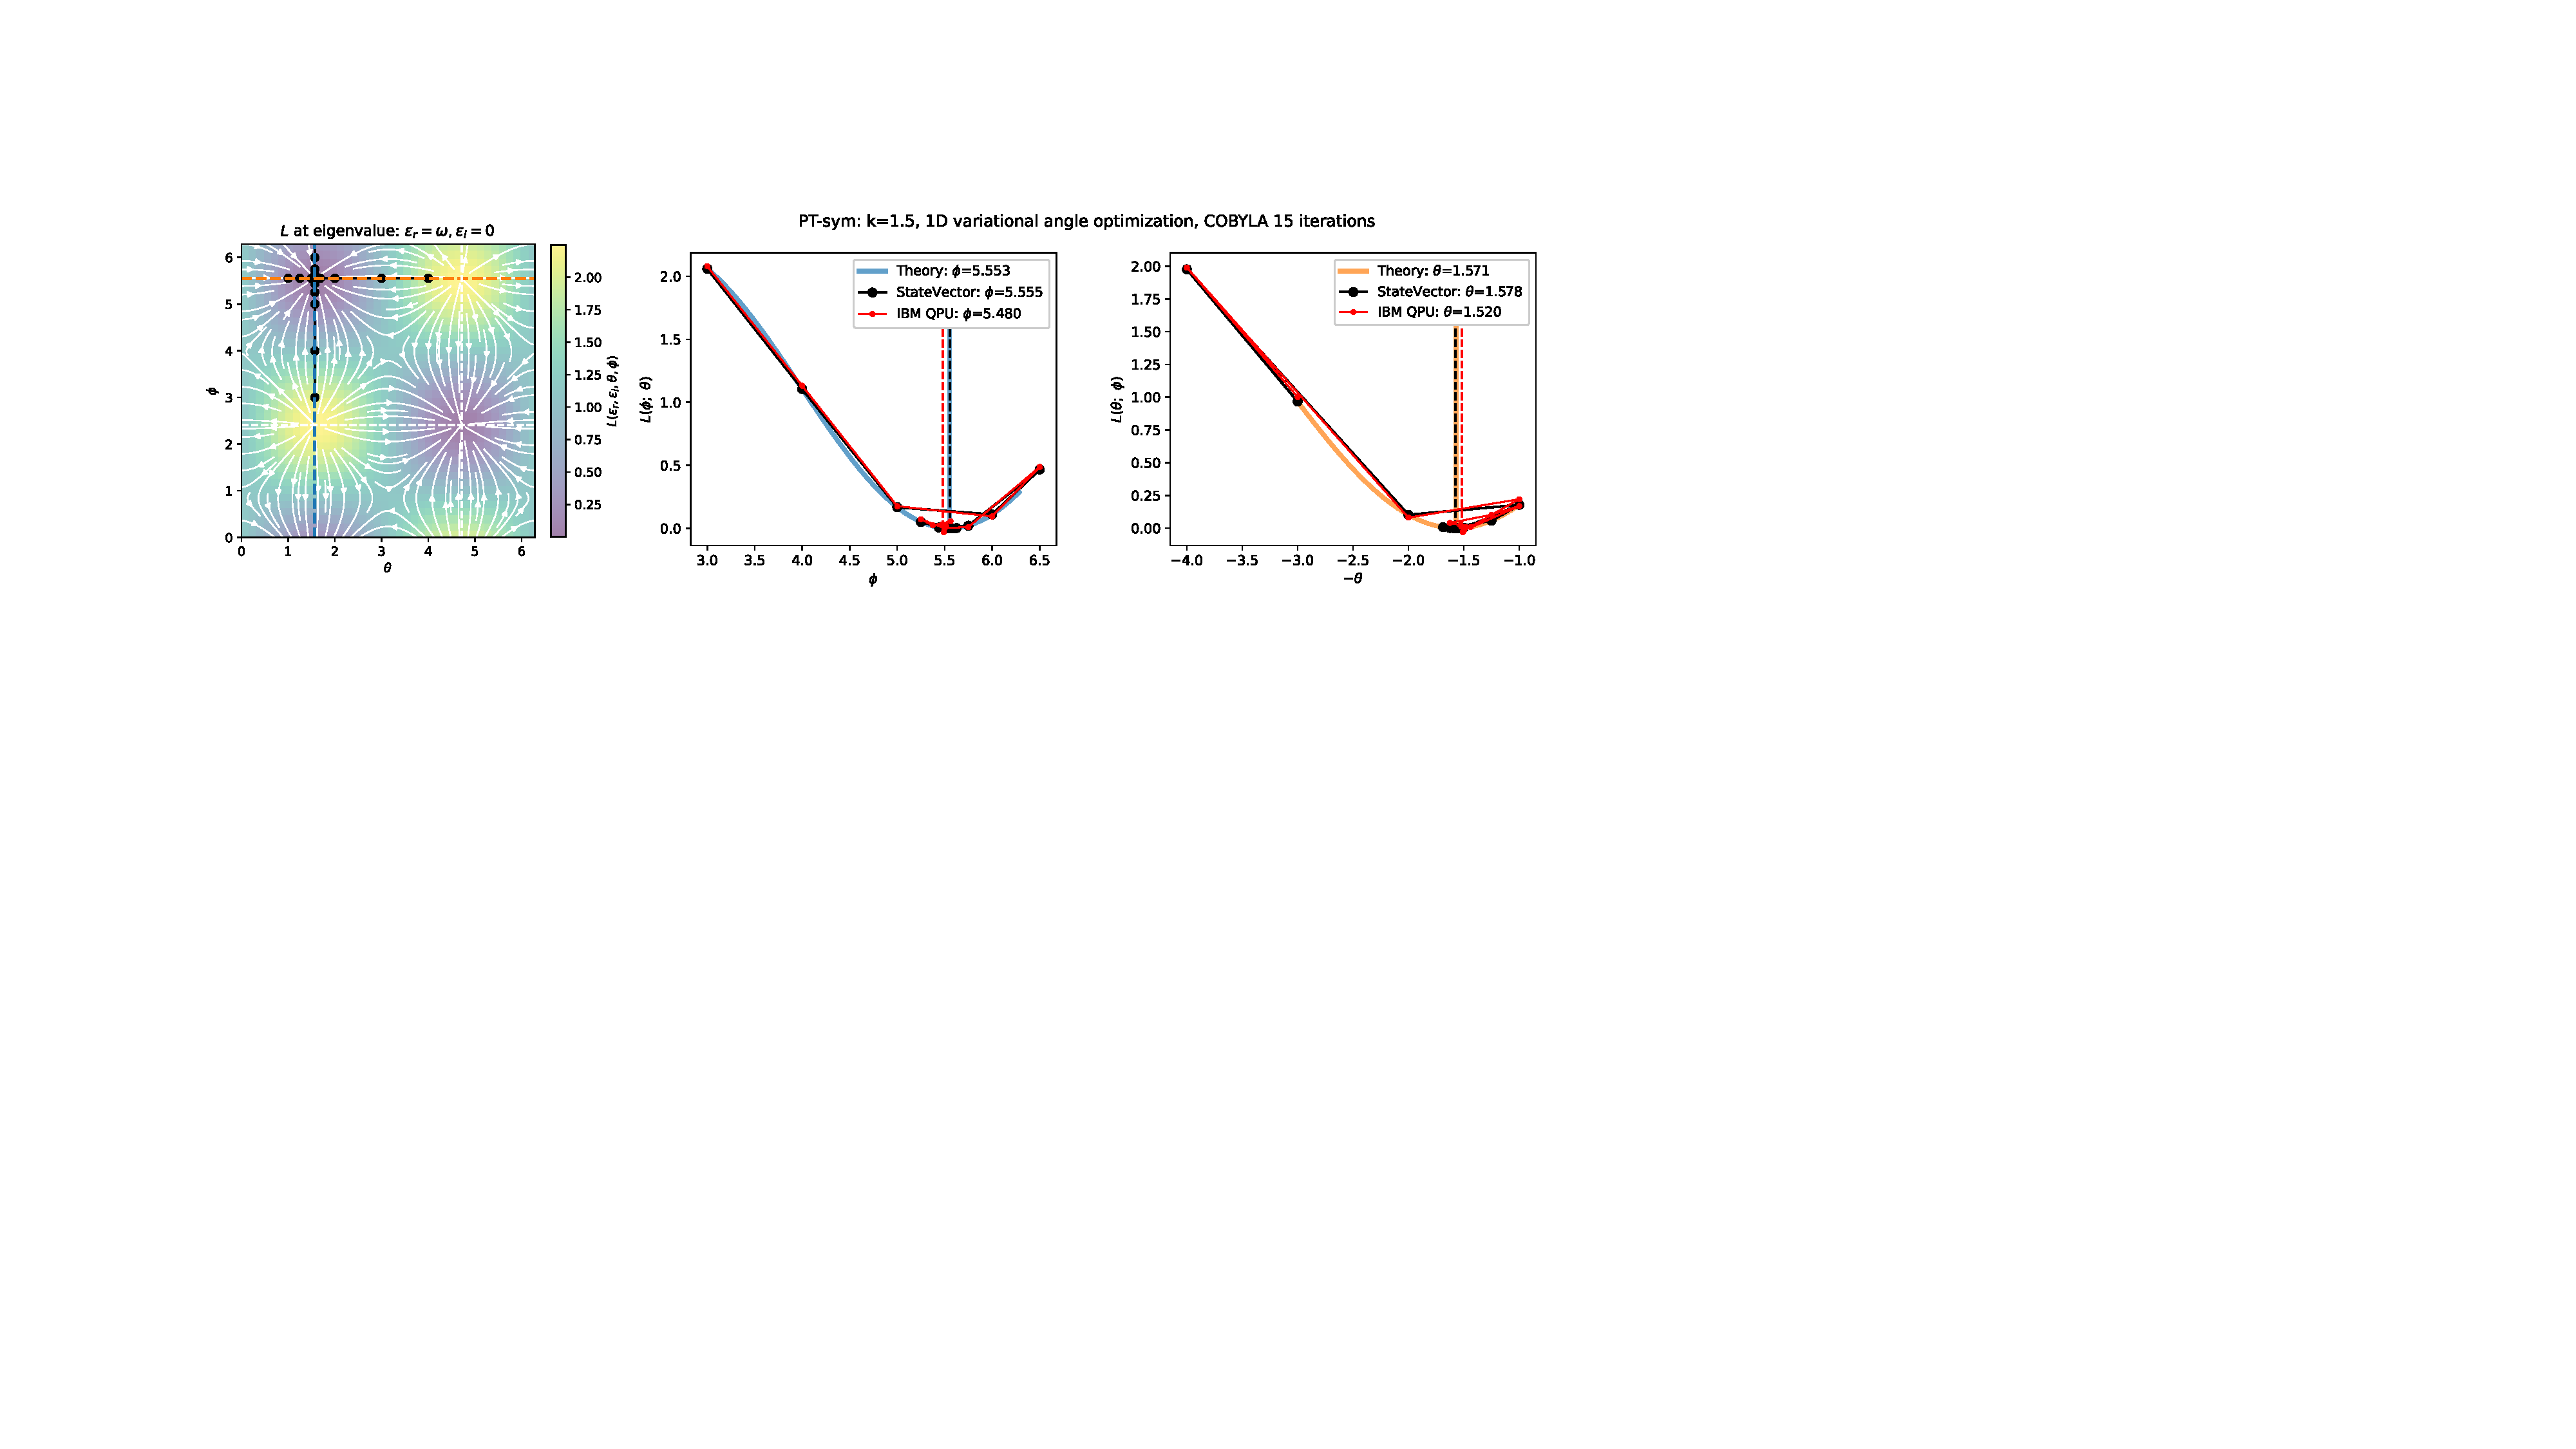
\includegraphics[width=0.8\linewidth]{figures/ptsym_opt.pdf}
    \caption{1D Optimization on IBM QPU.}
    \label{fig:ptsym_opt}
\end{figure}

In figure \ref{fig:ptsym_traject_opt4_cost_scipy} we run the full optimization loop for the 4 variational parameters. We specify a target optimization precision for the scipy optimizer or a maximum number of iterations for the loop. The two stages of optimizations can be seen through the abrupt change in the cost function.

\begin{figure}[!h]
    \centering
    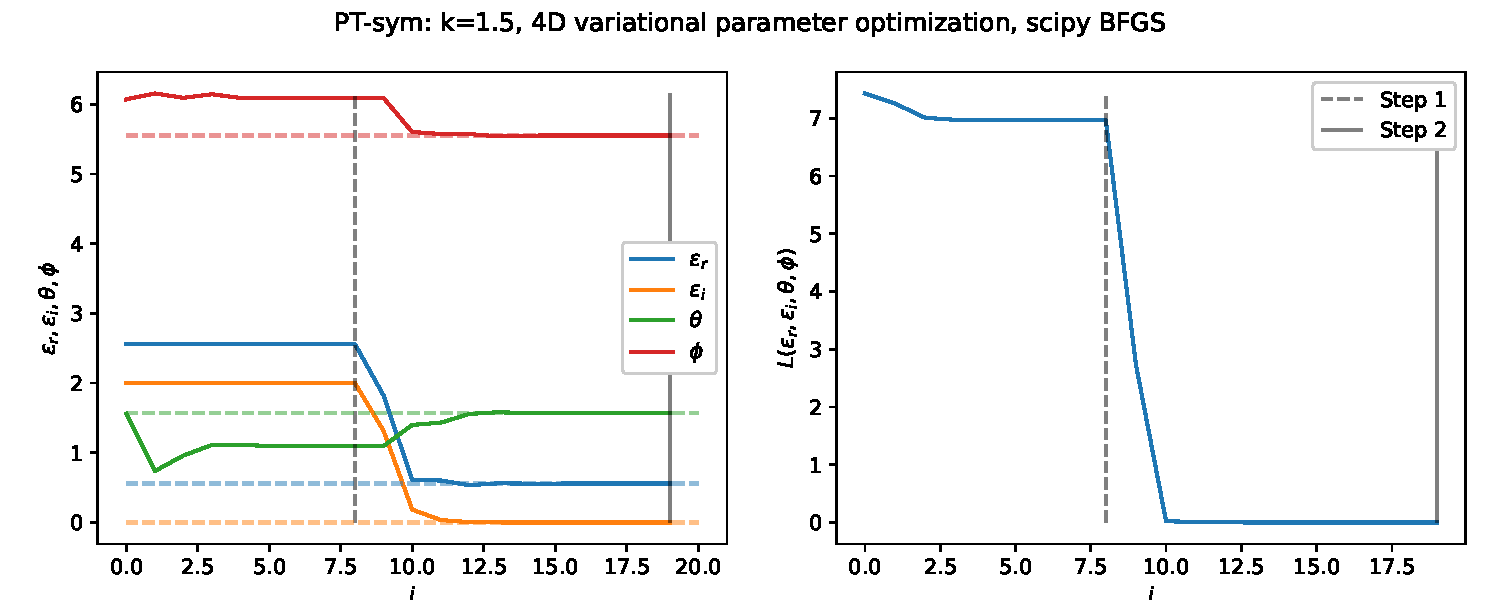
\includegraphics[width=0.8\linewidth]{figures/ptsym_traject_opt4_cost_scipy.pdf}
    \caption{Full optimization loop on simulator (no QPU).}
    \label{fig:ptsym_traject_opt4_cost_scipy}
\end{figure}


\end{document}